% !TeX spellcheck = de_DE
\documentclass[fontzize=12pt,paper=a4,twoside=false]{article}
\usepackage{german}
\usepackage{graphicx}
\usepackage{fullpage}

\title{Kurzwellenausbreitung}
\author{Konrad Gralher}

\begin{document}
\begin{titlepage}
    \bfseries\Huge\centering{
    Kurzwellenausbreitung\\
    Amateurfunklehgang 2021\\
    \vskip3cm
    \huge\itshape{
        Konrad Gralher\\
        }
    }    
    \begin{figure}
        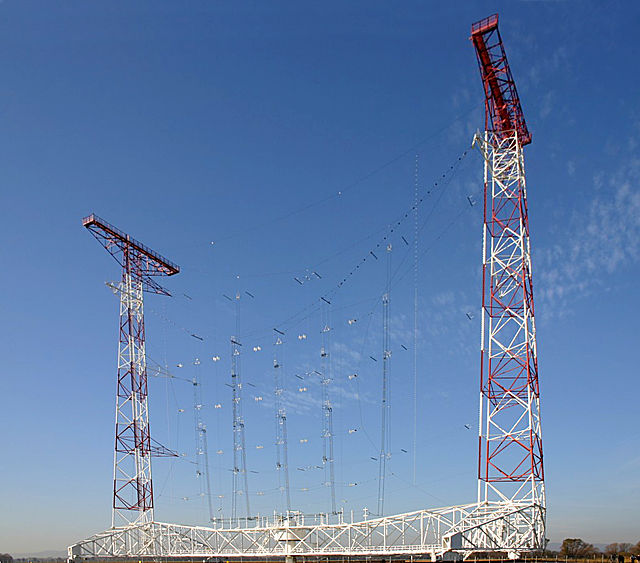
\includegraphics[]{assets/640px-Moosbrunn_SW_Antenna}
        \caption{Kurzwellenstation Moosbrunn}  
    \end{figure}        
\end{titlepage}

\part[]{Wellenausbreitung}

Die Sendungen im Kurzwellenbereich werden in der Ionosphäre reflektiert. 
Ukw besitzt diese Eigenschaften nicht, da die Wellen sich eher wie Licht ausbreiten(bedingt durch kleinere Wellenlänge). Durch Reflektionen der Kurzwelle an der Ionosphäre
sind deutlich größere Reichweiten möglich(DX Betrieb).
\vspace{0.1cm}
\subsection[]{Wellenarten}
Bei der Kurzwellenausbreitung spielen zwei Arten der Welle eine Rolle.
\begin{enumerate}
    \item Raumwelle
    \begin{itemize}
        \item bezeichnet alle sich im Raum ausbreitende Wellen(große Reichweite wenn in Skip Distanz)
    \end{itemize}
    \item Bodenwelle
    \begin{itemize}
        \item bezeichnet die sich am Boden mit der Erdkrümmung ausbreitende Welle (kleine Reichweite)
    \end{itemize}
\end{enumerate}

\end{document}